\documentclass{beamer}
\usepackage[utf8]{inputenc}

\usetheme{Madrid}
\usecolortheme{default}
\usepackage{amsmath,amssymb,amsfonts,amsthm}
\usepackage{txfonts}
\usepackage{tkz-euclide}
\usepackage{listings}
\usepackage{adjustbox}
\usepackage{array}
\usepackage{tabularx}
\usepackage{gvv}
\usepackage{lmodern}
\usepackage{circuitikz}
\usepackage{tikz}
\usepackage{graphicx}


\setbeamertemplate{page number in head/foot}[totalframenumber]


\title
{2.3.9}
\date{August 31, 2025}
\author 
{ADUDOTLA SRIVIDYA - EE25BTECH11006}

\begin{document}

\frame{\titlepage}


\begin{frame}{Question}
If vectors $\vec{a}$ and $\vec{b}$ are such that 
\[
|\vec{a}| = \frac{1}{2}, \quad |\vec{b}| = \frac{4}{\sqrt{3}}, \quad |\vec{a} \times \vec{b}| = \frac{1}{\sqrt{3}},
\]
then find $\vec{a} \cdot \vec{b}$.
\end{frame}


\begin{frame}{Formula}
We know that
\begin{align}
|\vec{a} \times \vec{b}| &= |\vec{a}||\vec{b}|\sin\theta \\
\vec{a} \cdot \vec{b} &= |\vec{a}||\vec{b}|\cos\theta
\end{align}
where $\theta$ is the angle between $\vec{a}$ and $\vec{b}$.
\end{frame}


\begin{frame}{Solution}
Substitute values:
\begin{align}
\frac{1}{\sqrt{3}} &= \left(\frac{1}{2}\right)\left(\frac{4}{\sqrt{3}}\right)\sin\theta \\
\sin\theta &= \frac{1}{2} \implies \theta = 30^\circ \ \text{or}\ 150^\circ
\end{align}

Now,
\begin{align}
\vec{a} \cdot \vec{b} &= \left(\frac{1}{2}\right)\left(\frac{4}{\sqrt{3}}\right)\cos\theta = \frac{2}{\sqrt{3}}\cos\theta
\end{align}
\end{frame}


\begin{frame}{Final Result}
For $\theta = 30^\circ$:
\[
\vec{a} \cdot \vec{b} = 1
\]
For $\theta = 150^\circ$:
\[
\vec{a} \cdot \vec{b} = -1
\]

\centering
\textbf{Therefore, $\vec{a} \cdot \vec{b} = \pm 1$.}
\end{frame}


\begin{frame}{Vector Plot}
\begin{figure}
    \centering
    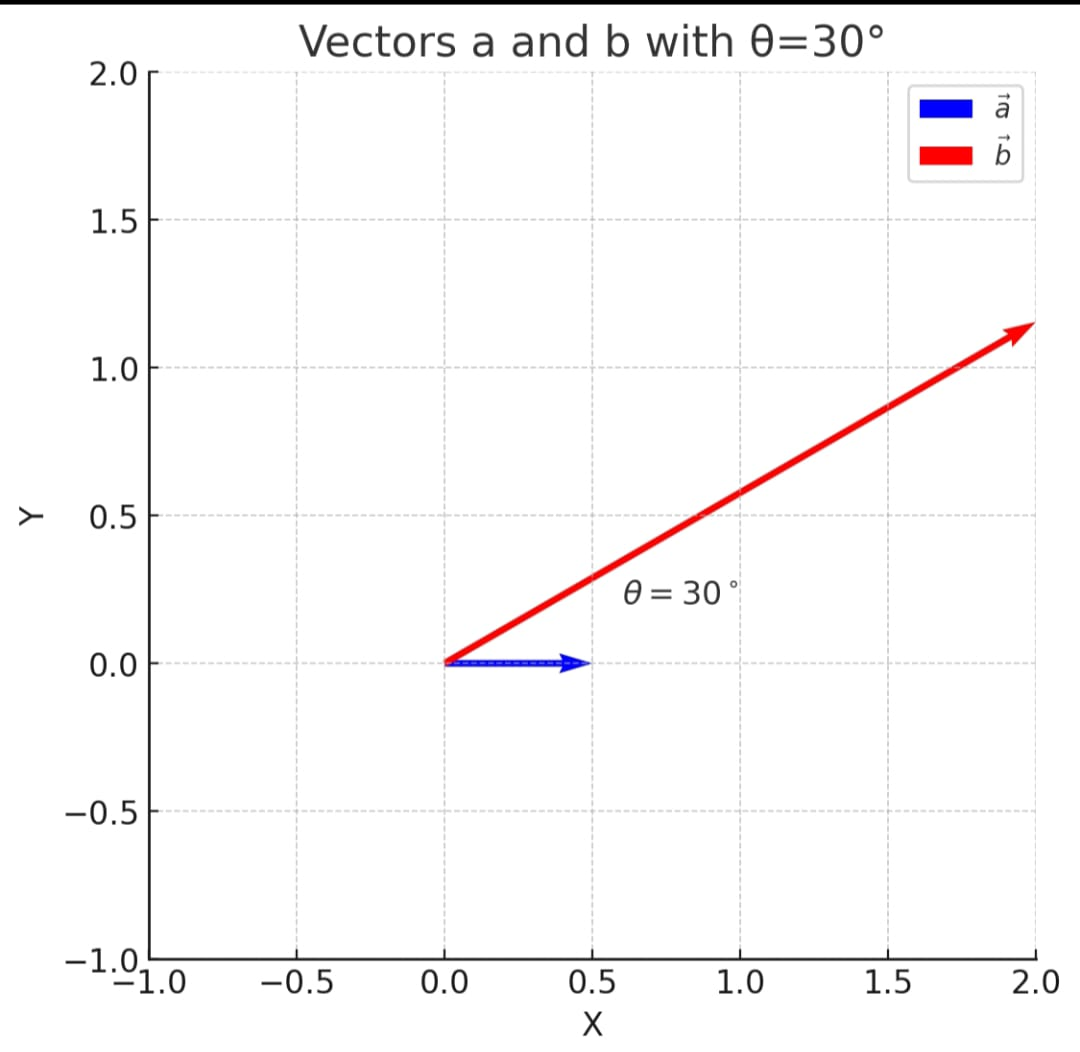
\includegraphics[width=0.5\columnwidth]{figs/fig2.3.9.jpeg}
    \caption{Vectors $\vec{a}$ and $\vec{b}$ with $\theta$}
    \label{fig:plot}
\end{figure}
\end{frame}

\begin{frame}[fragile]
\frametitle{C Code : Function Definition}
\begin{lstlisting}
#include<stdio.h>
#include<math.h>

float dotfinder(float a1, float a2, float a3, 
                float b1, float b2, float b3){

    float dot_product;
    float mod1;
    float mod2;
    float cosval;
    float angle;
    float result;
\end{lstlisting}
\end{frame}

\begin{frame}[fragile]
\frametitle{C Code : Function Logic}
\begin{lstlisting}
    dot_product = a1*b1 + a2*b2 + a3*b3;

    mod1 = sqrt(pow(a1,2) + pow(a2,2) + pow(a3,2));
    mod2 = sqrt(pow(b1,2) + pow(b2,2) + pow(b3,2));

    cosval = dot_product/(mod1 * mod2);

    angle = acos(cosval);   // angle between vectors

    result = dot_product;   // return a·b value

    return result;
}
\end{lstlisting}
\end{frame}

\begin{frame}[fragile]
\frametitle{Python Code : Setup}
\begin{lstlisting}[language=Python]
import numpy as np
import math

# Given magnitudes
a_mag = 1/2
b_mag = 4/np.sqrt(3)
cross_mag = 1/np.sqrt(3)

# sinθ = |a×b|/(|a||b|)
sin_theta = cross_mag/(a_mag*b_mag)
theta1 = math.degrees(math.asin(sin_theta))
theta2 = 180 - theta1
\end{lstlisting}
\end{frame}

\begin{frame}[fragile]
\frametitle{Python Code : Output}
\begin{lstlisting}[language=Python]
print("Possible angles:", theta1, "or", theta2)

# a·b = |a||b|cosθ
dot1 = a_mag*b_mag*math.cos(math.radians(theta1))
dot2 = a_mag*b_mag*math.cos(math.radians(theta2))

print("Possible values of a·b:", dot1, "or", dot2)
\end{lstlisting}
\end{frame}


\end{document}